% Sample of a report for an attack as requested at wednesday, 5 December 2018, mail "Assignemnt Lab 19"
\subsection{Attack Name}
% SCAPY program
\subsubsection{SCAPY program}
\lstinputlisting{scapy/SYNFlood.py}
With this program we are going to send every 5 milliseconds a SYN packet to an active port of the victim that we have found in the reconnaissance phase from the port 9999.\\
We have to wait that the session table of the victim reaches its edge, at this point the victim can no longer accept connections even if it is a legit ones.\par
I’ve also set the following settings on the victim pc to fill faster the session table:\\
\begin{lstlisting}
sysctl -w net.ipv4.tcp_syncookies=0
systcl -w net.ipv4.tcp_max_syn_backlog=256
\end{lstlisting}

% Wireshark presenting  the attacker's messages
\subsubsection{Victim's messages}

{\huge{TODO: import the Wireshark messages here}}\\

As shown after sending multiple SYN Flood the Victim starts responding with [RST,ACK] flags even to legit requests like the http request from ports 33648-33651 from the browser of the PC2.\par
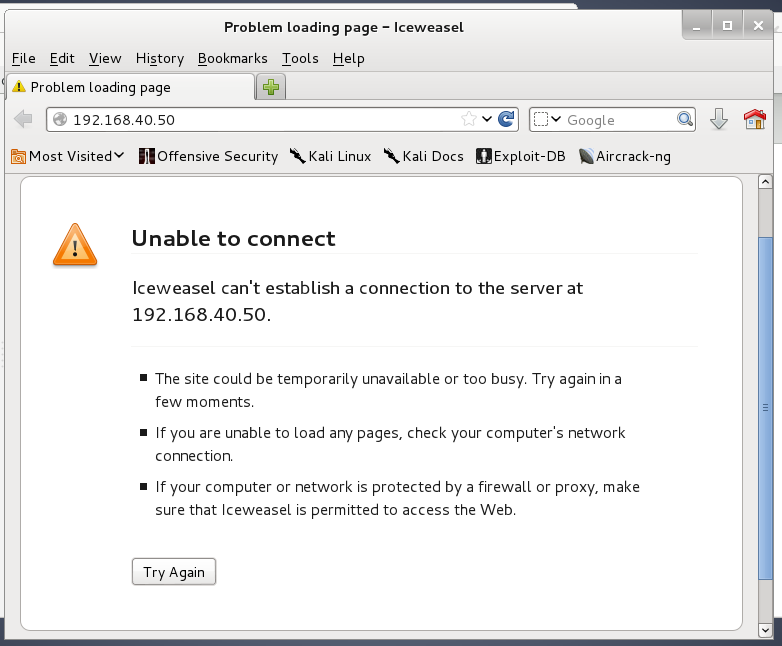
\includegraphics[width=16cm]{img/SYNFloodResult.png}\par

% Explanation of the result of the attack
\subsubsection{Attacker's messages}

{\huge{TODO: import the Wireshark messages here}}\\

In this case the attacker (PC2) is sending multiple SYN flags to the victim and in the last part of the messages is possible to see that even legit requests are denied.\par

% Method recommended to protect the Network against such an attack
\subsubsection{How to protect the network}
The possible solutions for prevent SYN Flood is to increase the backlog for TCP and to enable the syn cookies. Syn cookies are use to prevent syn flood by enlarging the SYN queue when it fills up. Now the server keeps responding with [SYN,ACK] but the server discards the SYN queue entries. When the server received an ACK flag it is able to reconstruct the SYN queue entry using informations encoded in TCP sequence number.\par
Another solution is to use a firewall. Some implementations of the firewall could be:\\
\begin{lstlisting}
iptables -A INPUT -p tcp -m state --state NEW -m recent --update --seconds 60 --hitcount 20 -j DROP
iptables -A INPUT -p tcp -m state --state NEW -m recent --set -j ACCEPT
\end{lstlisting}
In this way we limit the SYN request up to 20 per minute and we prevent the SYN flood. This is not best way to protect the network from Syn flood because in we can also drop legit requests coming from a network behind a nat.\par
Another implementation of the firewall could be:\\
\begin{lstlisting}
iptables -t mangle -I PREROUTING -p tcp -m tcp --dport 80 -m state --state NEW -m tcpmss ! --mss 536:65535 -j DROP
\end{lstlisting}
This rule checks 2 things. The first one is that the TCP Header contains the maximum size that the host wants to allow (hping, common attacking tool, doesn’t set this parameter by default). The second one is to check the port of the clients are in the range from 536 to 35535.\par
